\documentclass[a4paper,14pt]{extarticle} 
\usepackage[a4paper,top=1.5cm, bottom=1.5cm, left=2cm, right=1cm]{geometry}
%\usepackage[T2A]{fontenc}
%\usepackage[english, russian]{babel}
\usepackage{graphicx}
\graphicspath{{./pics/}}
\DeclareGraphicsExtensions{.pdf,.png,.jpg}

\usepackage{fontspec}
\setmainfont{Times New Roman}
\setsansfont{FreeSans}
\setmonofont{FreeMono}
\renewcommand{\baselinestretch}{1.5}
\usepackage{polyglossia}
\setdefaultlanguage{russian}
\setotherlanguages{english,russian}
\usepackage{setspace}
\usepackage[many]{tcolorbox}
\usepackage{pdfpages}

\begin{document}

    \begin{center}
        \thispagestyle{empty}
        \begin{singlespace}
        ФЕДЕРАЛЬНОЕ АГЕНТСТВО СВЯЗИ

        ФЕДЕРАЛЬНОЕ ГОСУДАРСТВЕННОЕ БЮДЖЕТНОЕ ОБРАЗОВАТЕЛЬНОЕ

        УЧРЕЖДЕНИЕ ВЫСШЕГО ОБРАЗОВАНИЯ

        «САНКТ-ПЕТЕРБУРГСКИЙ ГОСУДАРСТВЕННЫЙ УНИВЕРСИТЕТ ТЕЛЕКОММУНИКАЦИЙ ИМ. ПРОФ. М.А. БОНЧ-БРУЕВИЧА»

        (СПбГУТ)
        \end{singlespace}
        \vspace{-1ex}
        \rule{\textwidth}{0.4pt}
        \vspace{-5ex}

        Факультет \underline{Инфокоммуникационных сетей и систем}

        Кафедра \underline{Защищенных систем связи}
        \vspace{10ex}

        \textbf{Лабораторная работа №5}

    \end{center}
    \vspace{4ex}
    \begin{flushright}
    \parbox{8cm}{
    \begin{flushleft}
        Выполнил:

        \underline{Громов А.А., ИКТЗ-83} \hfill \rule[-0.85ex]{0.1\textwidth}{0.6pt}\\
        \vspace{-1ex}
        \footnotesize \textit{ (Ф.И.О., № группы) \hfill (подпись)} \normalsize

        Проверил:

        \underline{Гельфанд А.М.} \hfill \rule[-0.85ex]{0.1\textwidth}{0.6pt}\\
        \vspace{-1ex}
        (\footnotesize \textit{уч. степень, уч. звание, Ф.И.О.) \hfill (подпись)} \normalsize

    \end{flushleft}
    }
    \end{flushright}
    \begin{center}
        \vfill
        Санкт-Петербург

        2020

        \end{center}

    \newpage

    1. Перечислите любые 3 протокола, которые могут быть отображены в столбце
    Protocol (Протокол) при отключенном фильтре пакетов и показанном на рис. 3.
    Сколько времени прошло от момента отправки сообщения GET протокола HTTP до
    получения ответного сообщения OK? (По умолчанию, значения поля Time (Время)
    в окне списка представляет собой время в секундах от начала трассировки. Вы
    можете поменять вид этого поля по вашему желанию, выбрав в меню View (Вид)
    пункт Time Display Format (Формат отображения времени) и затем указав
    подходящее представление времени.)

    Протоколы: UDP, TCP, ARP, DNS.\\
    Прошло ~0,12с от отправки get запроса, до получения ответного сообщения ОК.

    2. Какой IP-адрес у сервера gaia.cs.umass.edu(также известного как \\
    www.net.cs.umass.edu)? Каков адрес вашего компьютера?

    IP-адрес сервера gaia.cs.umass.edu: 128.119.245.12

    IP-адрес компьютера: 192.168.0.33

    3. Распечатайте сообщения протокола HTTP (GET и OK), полученные вами при ответе
    на предыдущий вопрос. Для этого выберите команду меню File -> Print (Файл ->
    Печать), установите переключатели в положение Selected Packet Only (Только
    выбранный пакет) и Print as displayed (Печатать в формате отображения),
    соответственно, и затем нажмите кнопку OK.
    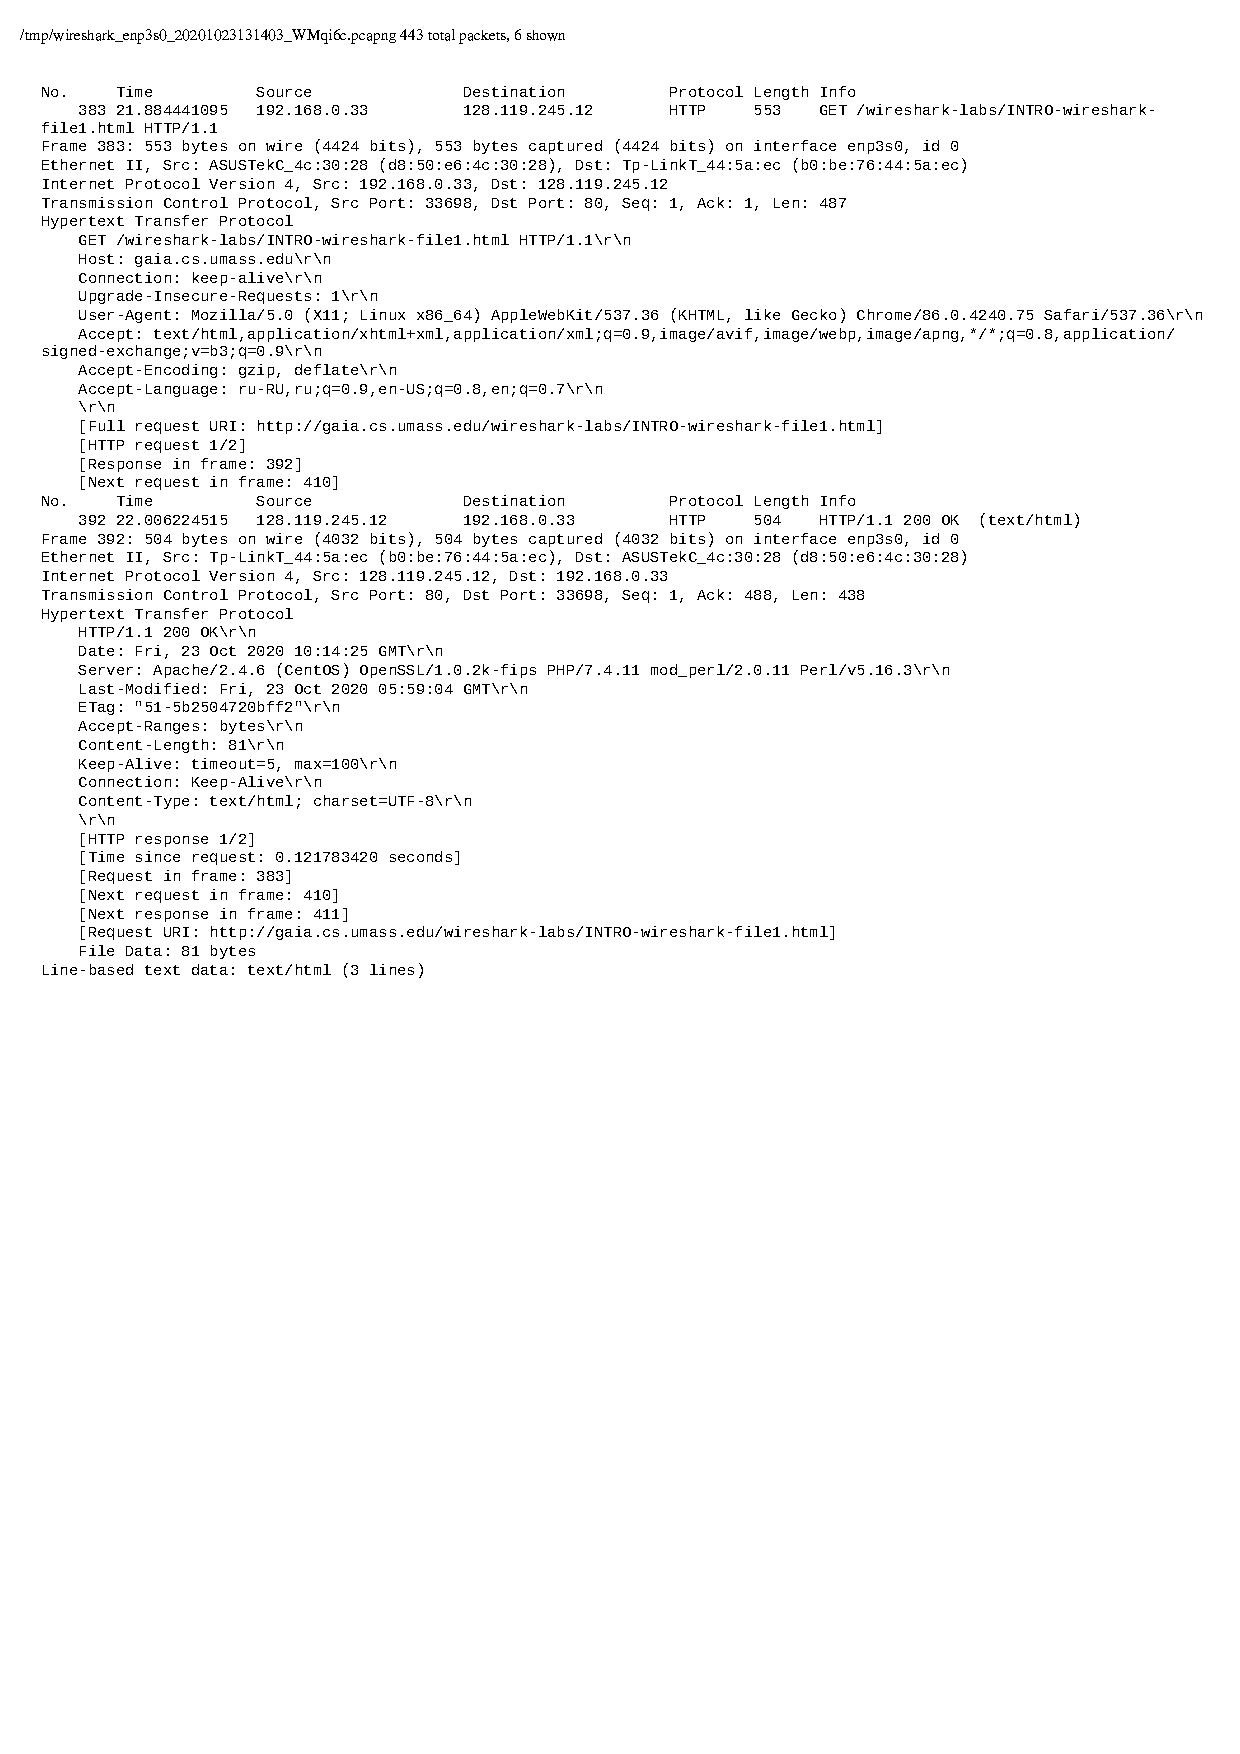
\includepdf[pages=1,pagecommand={},width=\textwidth]{get_ok.pdf}
\end{document}